\documentclass[twoside, 12pt]{article}
\usepackage[utf8]{inputenc}
\usepackage[portuguese]{babel}
\usepackage[default]{opensans} % tipo calibri

\usepackage[percent]{overpic}
\usepackage{geometry}
\usepackage{fancyhdr} % Deve ser depois de geometry
\usepackage{calc}
\usepackage{afterpage}
\usepackage{svg}

\usepackage{hyperref}
\usepackage{graphicx}

%%%%%%%%%%%%%%%%%%% Definições do usuário %%%%%%%%%%%%%%%%%%%%%%%

% Defina as margens esquerda, direita, topo e baixo
\newlength{\margemesq}  \setlength{\margemesq} {2.5cm}
\newlength{\margemdir}  \setlength{\margemdir} {2.5cm}
\newlength{\margemtopo} \setlength{\margemtopo}{1.5cm}
\newlength{\margembaix} \setlength{\margembaix}{2.5cm}
% Atenção ao aviso de fancy header. Ele que recomendou essa altcabec.
% Recomendamos não deixar menor do que isso, só maior. Se quiser um
% cabeçalho menor (para todas as páginas que não a primeira), ajuste
% também o tamanho da imagem "logo"
\newlength{\altcabec}   \setlength{\altcabec}  {22.71pt}

%%%%%%%%%%%%%%%%%%%%%%%%%%%%%%%%%%%%%%%%%%%%%%%%%%%%%%%%%%%%%%%%%

\geometry{
  a4paper,
  includeheadfoot,
  lmargin=\margemesq,
  rmargin=\margemdir,
  tmargin=\margemtopo,
  bmargin=\margembaix,
  headheight=\altcabec,
}

%%%%%%%%%% Cabeçalho e rodapé %%%%%%%%%%%%%%%%

\fancyhf{}
\fancypagestyle{primeirapagina}{
  \setlength{\headheight}{0mm}
  \setlength{\headsep}{0mm}
  \fancyhead[LE,RO]{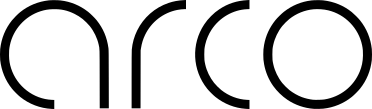
\includegraphics[width=2.3cm]{logo}}
  \fancyfoot[LE,RO]{\thepage}
}

\fancypagestyle{normal}{
  \fancyhead[LE,RO]{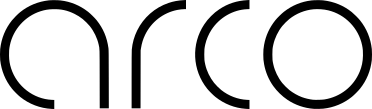
\includegraphics[width=2.3cm]{logo}}
  \fancyfoot[LE,RO]{\thepage}
}

\pagestyle{normal}

%%%%%%%%%%%%%%%%%%%%%%%%%%%%%%%%%%%%%%%%%%%%%%

% CABEÇALHO ARCO (provavelmente você não quer mexer nisso)
% titulo
\newlength{\largtit} \setlength{\largtit}{105mm}
\newlength{\alttit} \setlength{\alttit}{8mm}
% infos
\newlength{\larginfo} \setlength{\larginfo}{175mm}
\newlength{\divisaoinfo} \setlength{\divisaoinfo}{120mm}
\newlength{\altinfo} \setlength{\altinfo}{5mm}

% Desconta espaço horizontal (posição do cabeçalho arco é fixa)
\newlength{\subtraih} \setlength{\subtraih}{-\margemesq + 0.75cm}

\renewcommand{\headrulewidth}{0pt} % não usar a linha padrão do cabeç.
\renewcommand{\footrulewidth}{0pt}

\newcommand{\cabecalho}[4] {
  \thispagestyle{primeirapagina}
  \hspace*{\subtraih}
  % \vspace*{\subtraiv}
  \begin{overpic}[abs, unit=1mm, width=16.347cm + 2cm]{cabecalho}
    % Título
    \put (3.3,22) {
      \begin{minipage}[c][\alttit][c]{\largtit}
        #1
      \end{minipage}
    }
    % Subtítulo
    \put (3.3,12.9) {
      \begin{minipage}[c][\alttit][c]{\largtit}
        #2
      \end{minipage}
    }
    % Informações
    \put (3.3,3.7) {
      \begin{minipage}[c][\altinfo][c]{\divisaoinfo}
        #3
      \end{minipage}
      \begin{minipage}[c][\altinfo][c]{\larginfo - \divisaoinfo}
          #4
      \end{minipage}
    }
  \end{overpic}
  \hspace*{0mm}
  \bigskip
}


%%%%%%%%%%%%%%% Início do documento %%%%%%%%%%%%%%%%%%%%%%%%%

\begin{document}

\cabecalho{
  \huge 03 - Congruência
}{
  Matemática
}{
  9º ano
}{
  \begin{flushright}
    abr/2021
  \end{flushright}
}

Nessa atividade vamos investigar a ideia de igualdade entre figuras.
Veja as duas figuras abaixo:

\begin{center}
  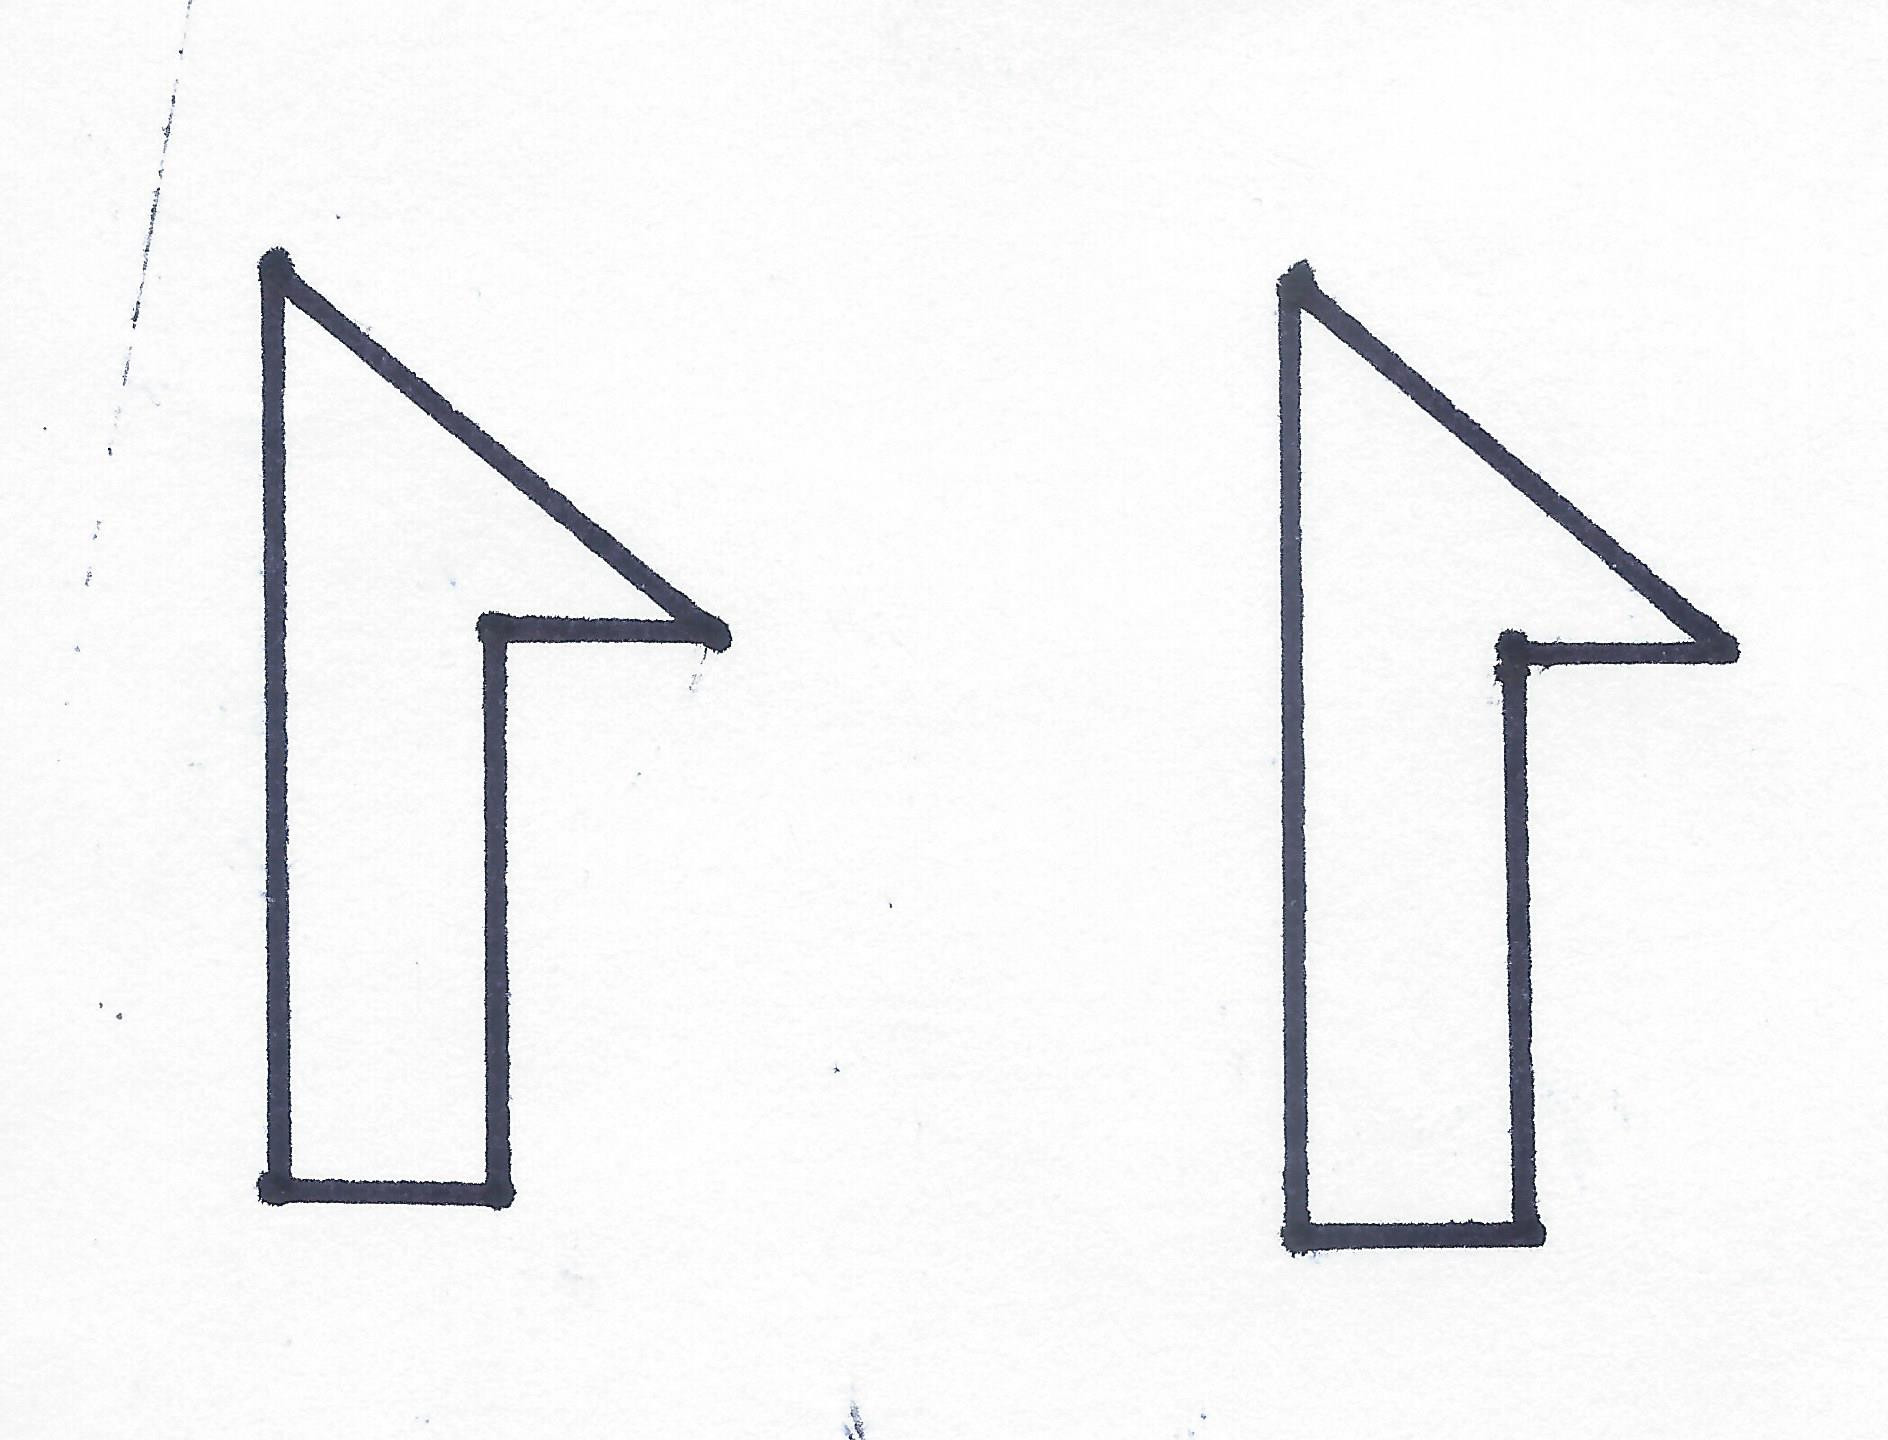
\includegraphics[height=0.2\textheight]{img/03-1}
\end{center}

Parece razoável dizer que elas são iguais. Elas tem a mesma forma e o
mesmo tamanho. E essas duas?

\begin{center}
  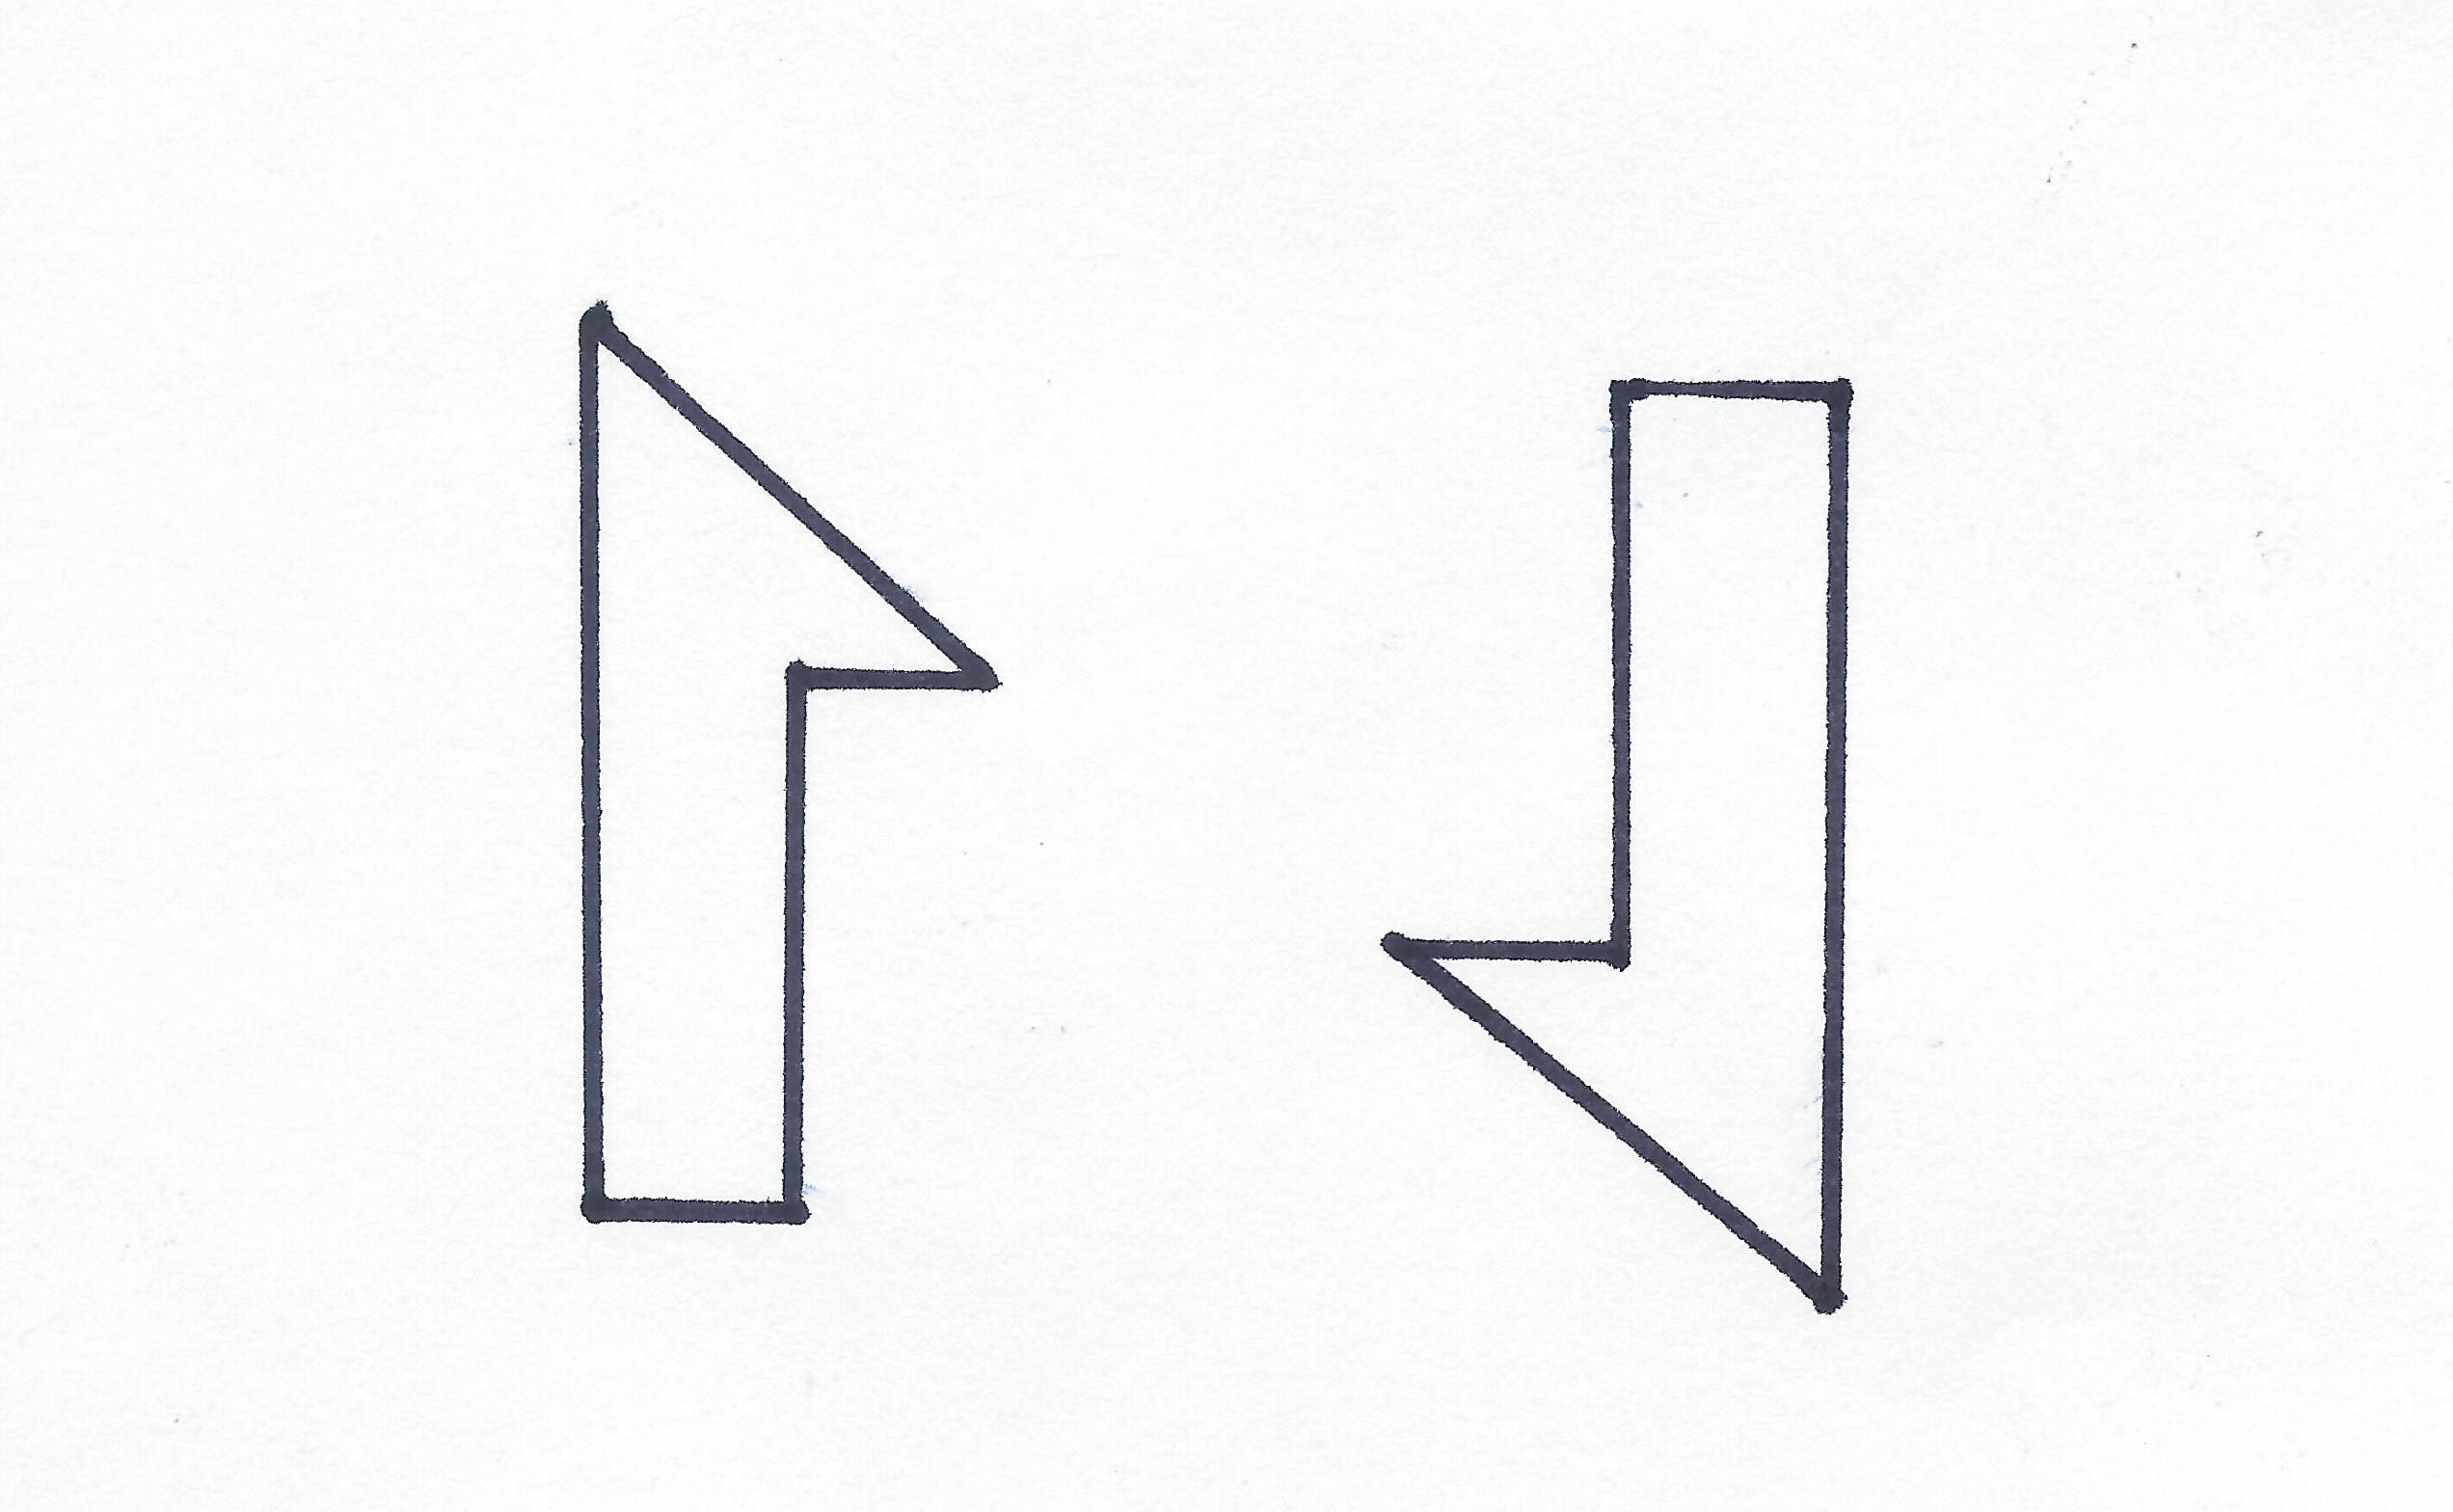
\includegraphics[height=0.2\textheight]{img/03-2}
\end{center}

Parece razoável também que elas sejam iguais, afinal, parece que a gente
só girou uma delas e chegou na outra. E essas?

\begin{center}
  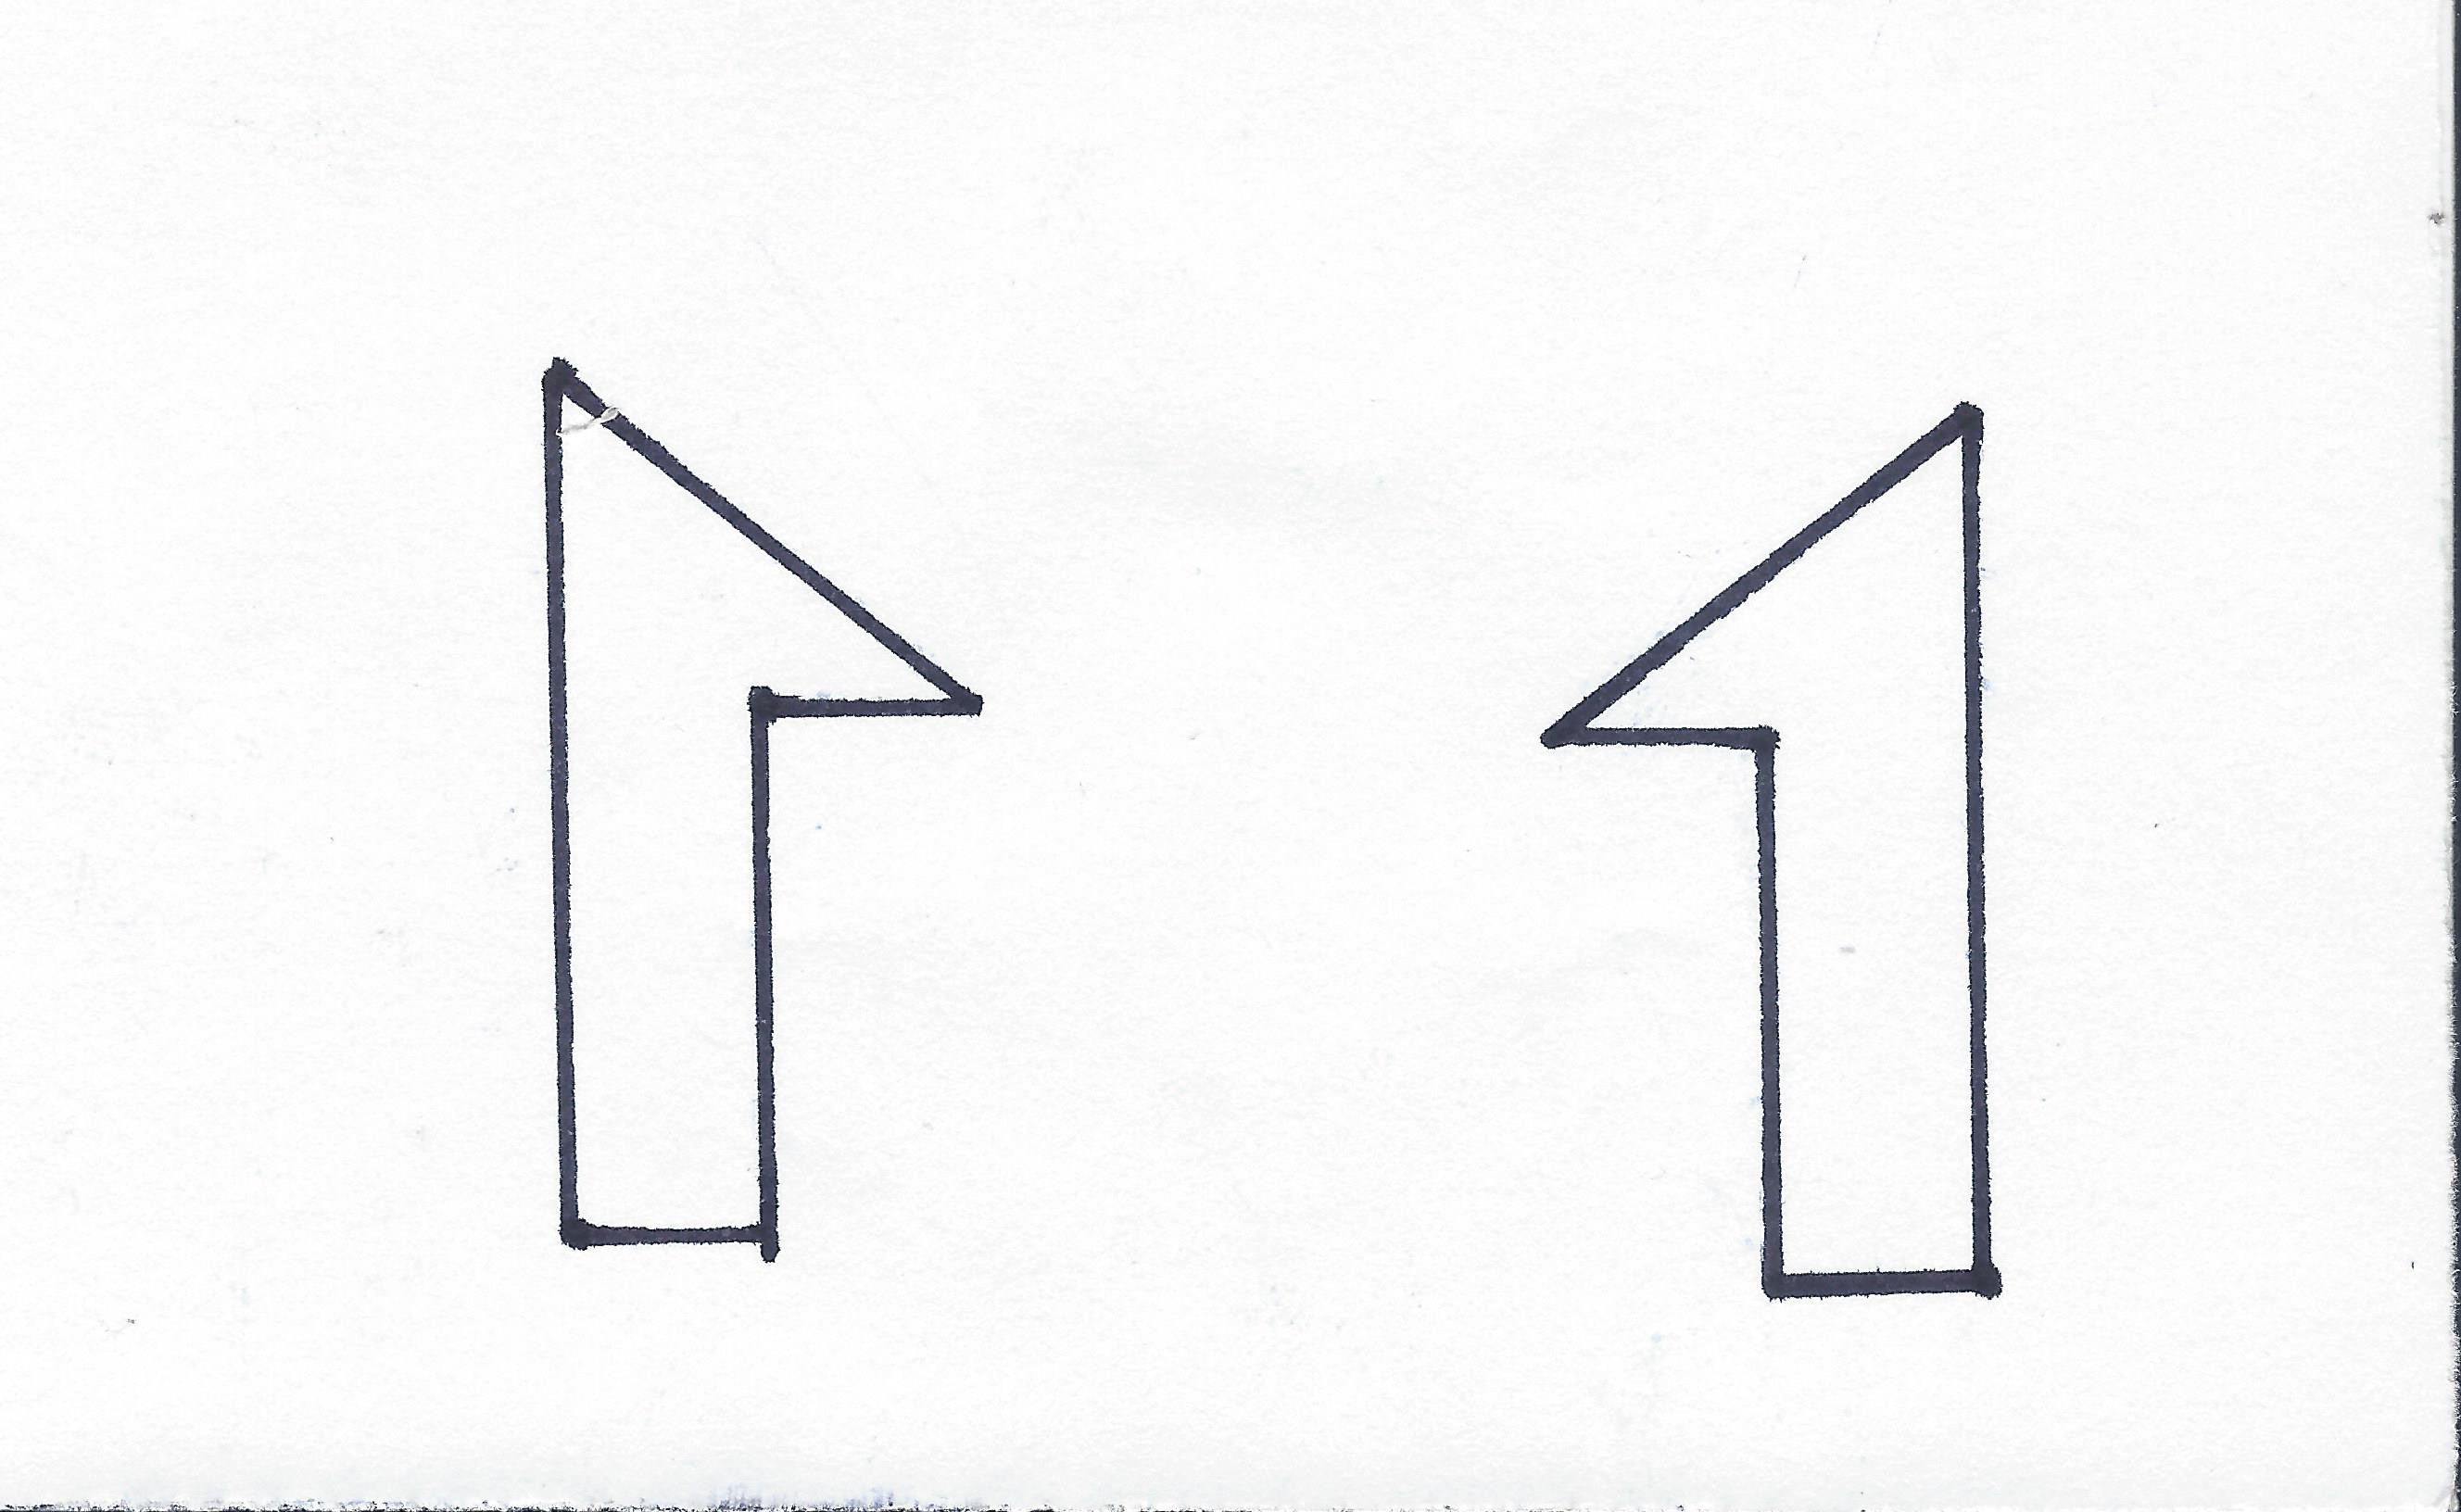
\includegraphics[height=0.2\textheight]{img/03-3}
\end{center}

Aqui já ficamos mais na dúvida. Por um lado, parece que elas tem a mesma
forma, por que se eu virar uma figura eu chego na outra. Mas uma aponta
para a direita e outra pra esquerda... E essas?

\begin{center}
  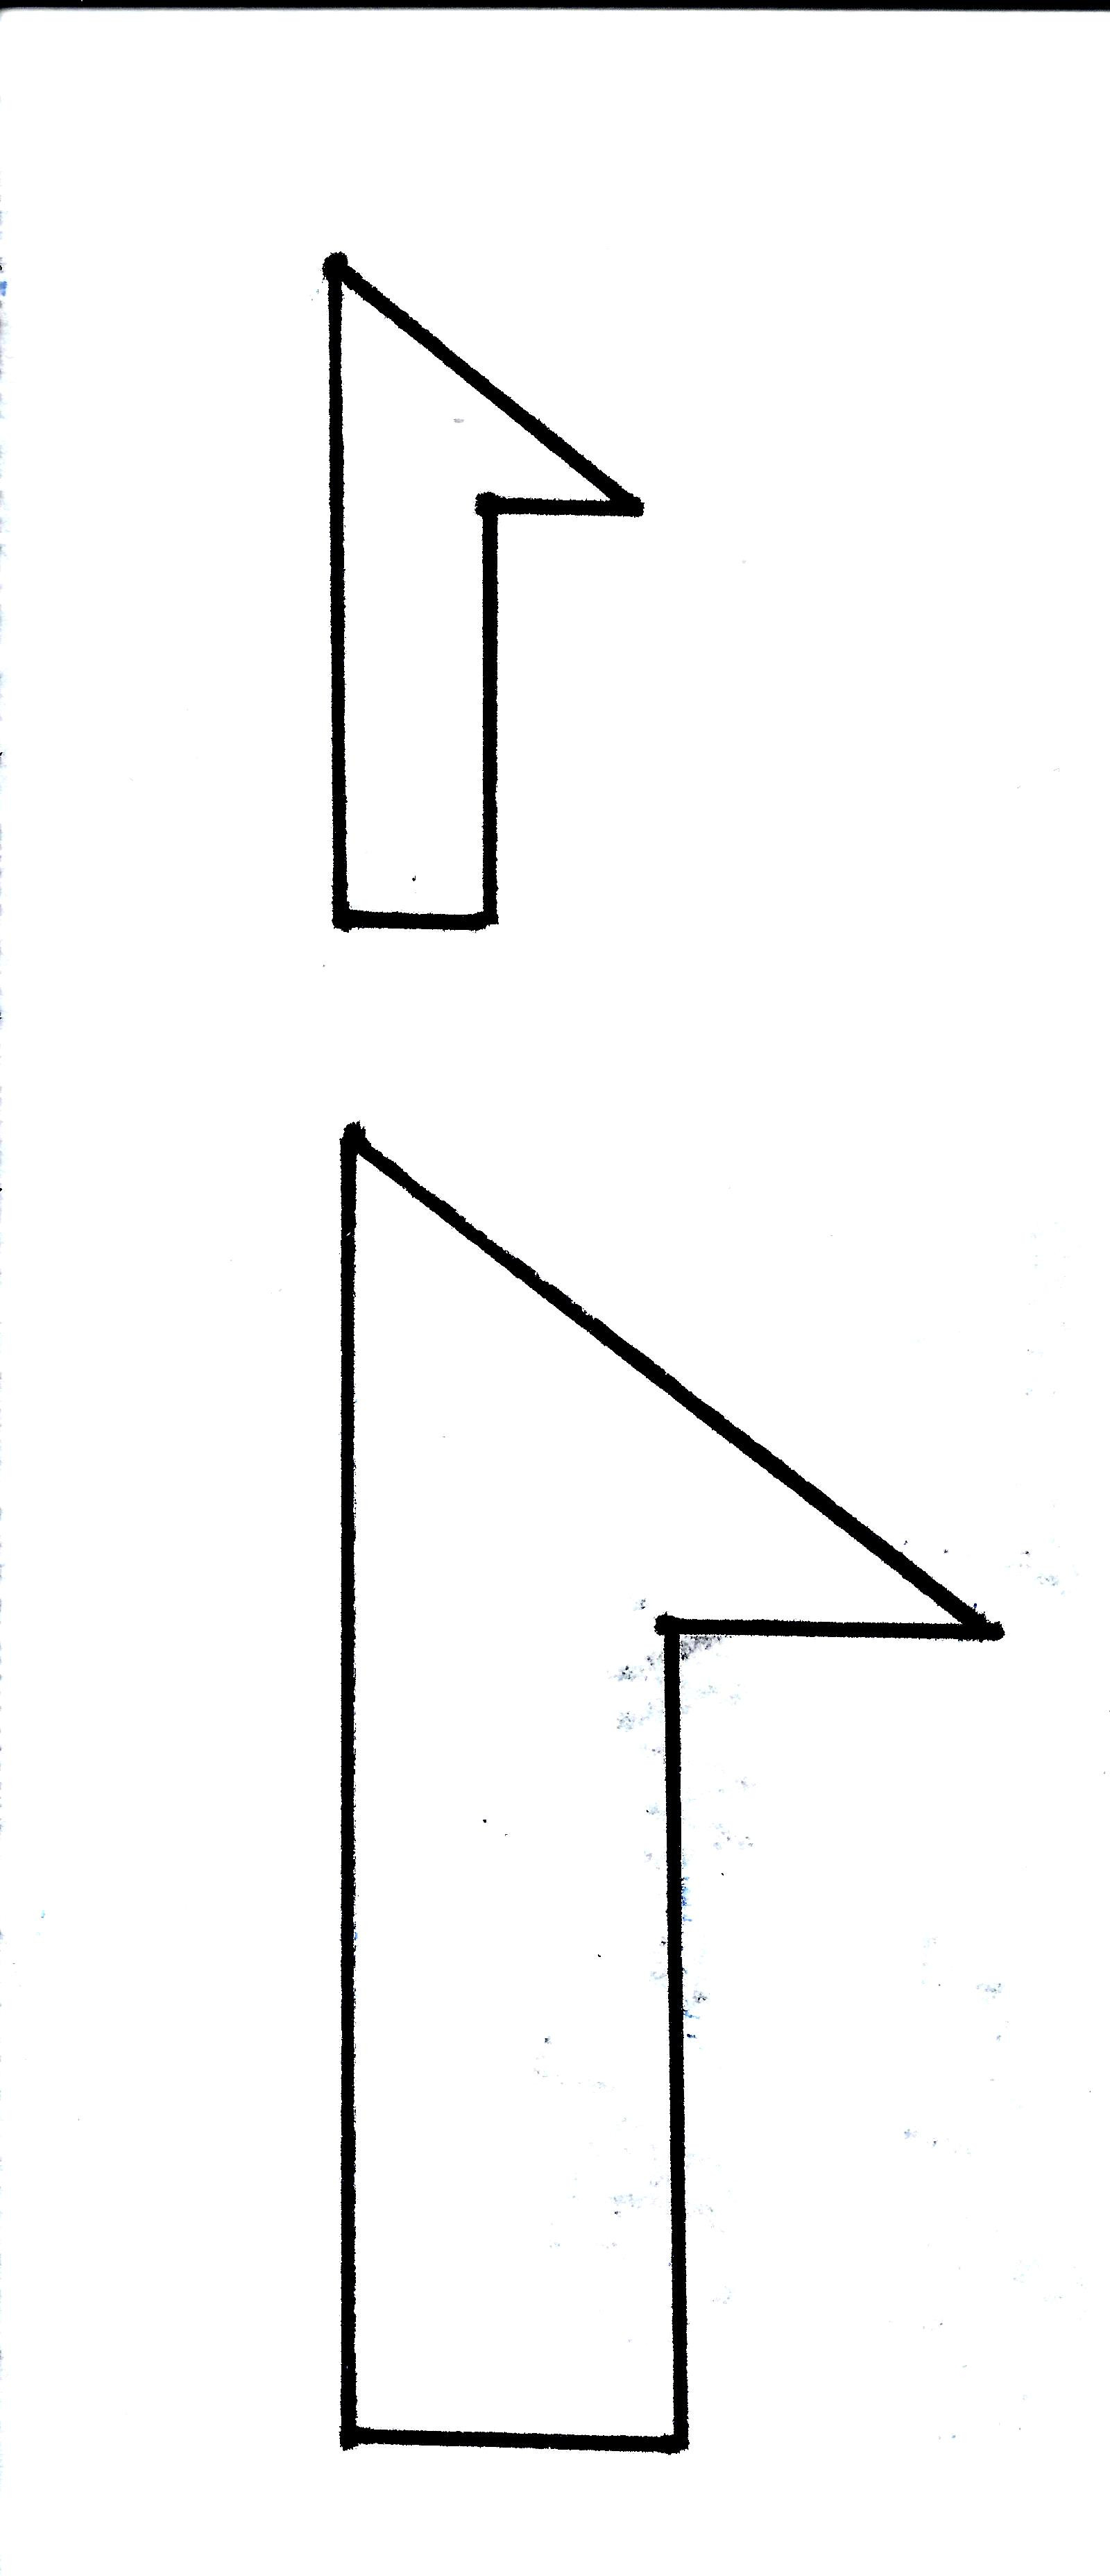
\includegraphics[height=0.2\textheight]{img/03-4}
\end{center}

Bom, elas ainda são parecidas, mas uma é maior que a outra. Será que
elas são iguais?

\section{Congruência}

Em vez de ficar tentando responder essa pergunta, que parece não ter uma
resposta definitiva, vamos apresentar outro conceito. Em geometria,
dizemos que duas figuras são \textbf{congruentes} se elas tem a mesma
forma e o mesmo tamanho.

As seguintes figuras são congruentes, porque têm o mesmo tamanho e
forma:

\begin{center}
  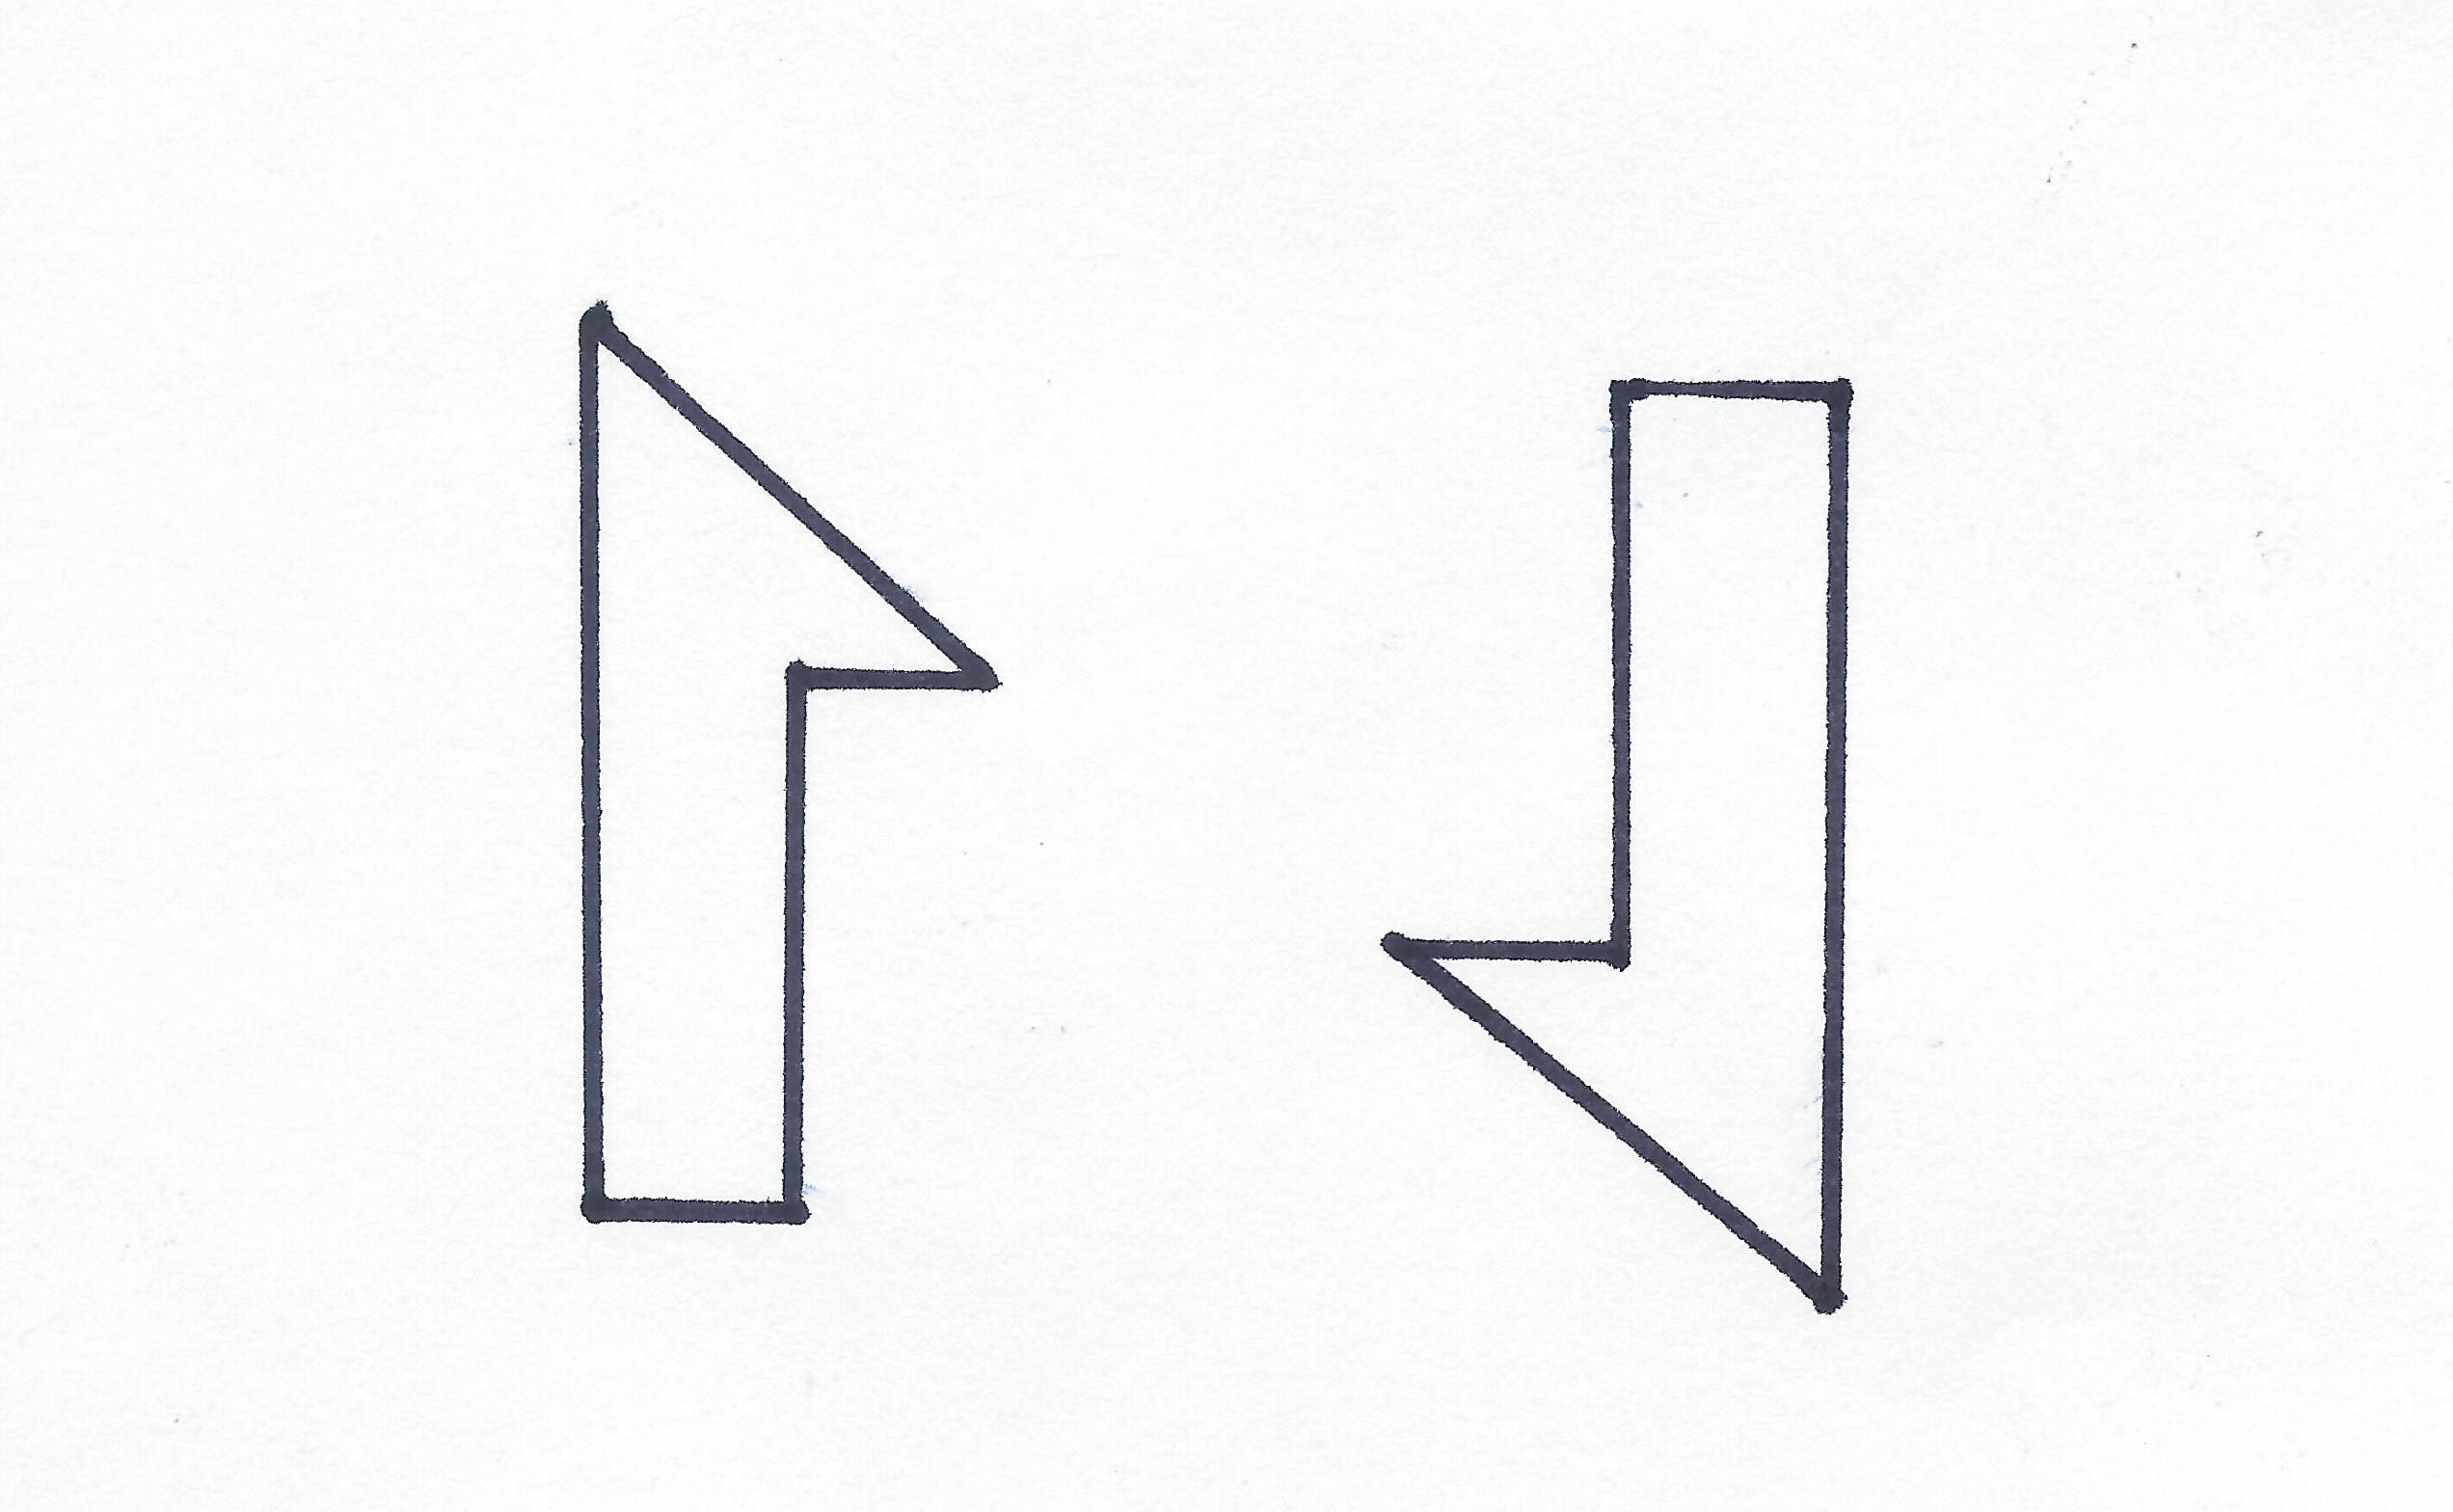
\includegraphics[height=0.2\textheight]{img/03-2}
\end{center}

Mas essas não, porque têm tamanhos diferentes.

\begin{center}
  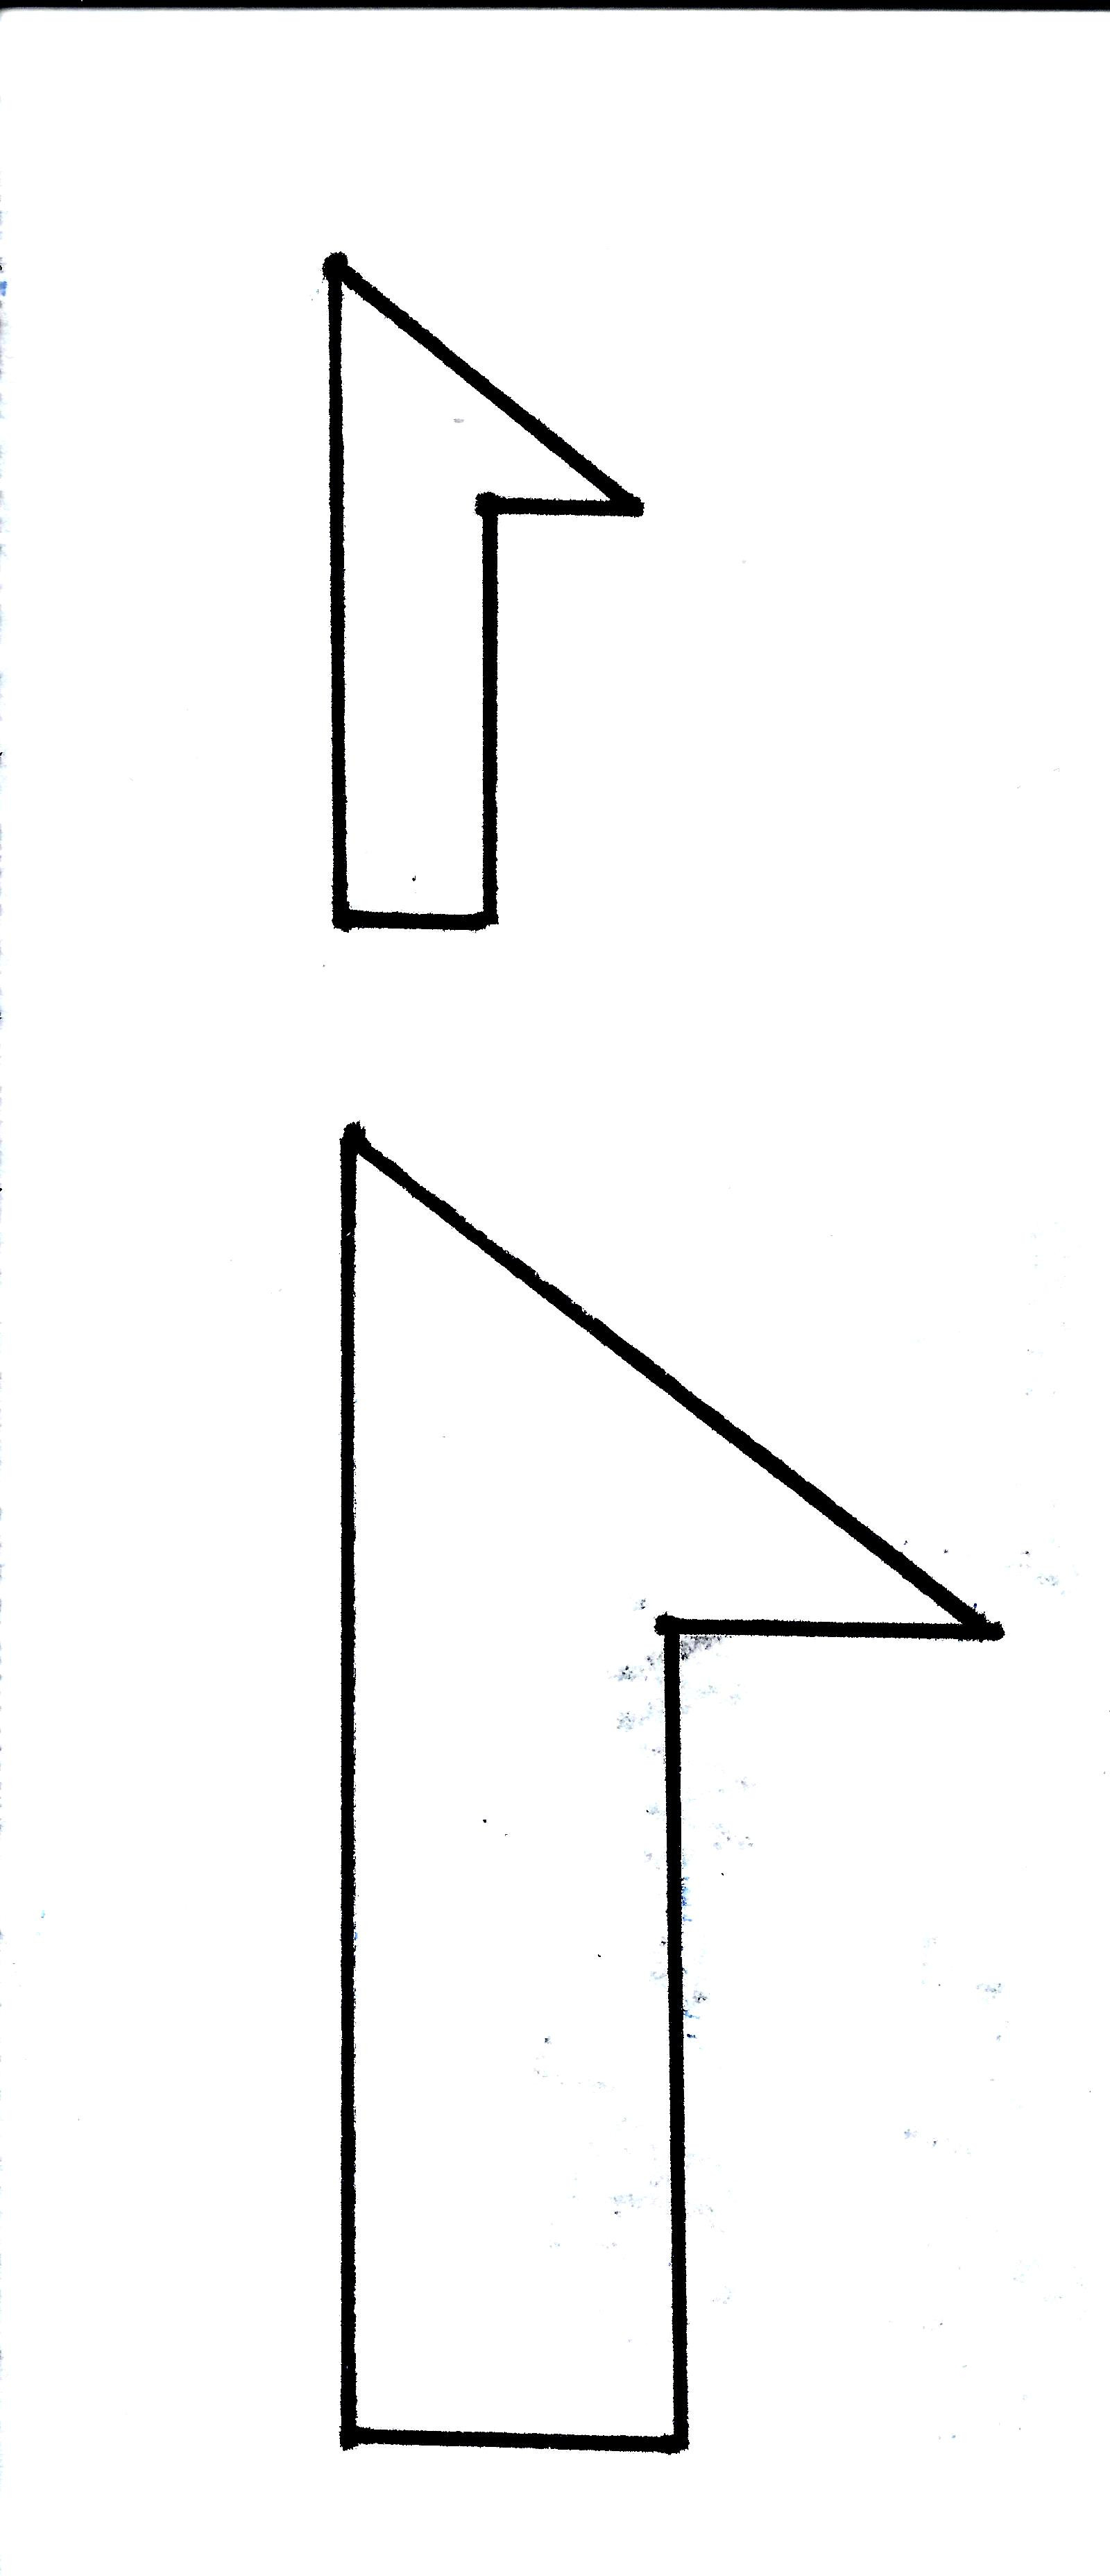
\includegraphics[height=0.2\textheight]{img/03-4}
\end{center}

\begin{center}
  \fbox {\parbox{0.7\textwidth}{
    \large Duas figuras são ditas congruentes se têm a mesma
    \bf{forma} e mesmo \bf{tamanho}
  }}
\end{center}

\bf{Exercício 1}

Faça a seguinte atividade no geogebra: \url{geogebra.org/m/gadrnmzm}.
Registre sua resolução com \emph{printscreens} e poste-os no Google Sala
de Aula

\end{document}

